\originalchapter{8.012 公开考试: 完整题面与核对解答}\label{ch:exams}
以下四卷均为 8.012 Fall 2008 页面实际公开材料, 原作者 Adam Burgasser. 三次期中各 90 分钟, 期末 150 分钟; 均要求完成全部题目、写出过程、圈出答案, 禁止书籍、笔记、计算器及电脑, 允许官方提供的公式表. 期中各五题, 期末七题. 保留全部选择项、小问及 bonus. 原试卷的答题空白页不复制. 每段解答是本册中文推导, 已对照公开官方答案; 标明的补充、条件澄清及更正为 AI 独立工作, 不能当作官方原话. 与题设有关的原图几何以文字或新图完整说明. 第三卷内页误印 Fall 2007, 封面和 OCW 所属课程为 Fall 2008, 此处保留记录而不擅改历史.

\originalsection{期中一: 牛顿定律与运动学}
原分值依次为 10、30、20、20、20, 总分 100.
\begin{exercise}
原题 1, 快速选择. (a) 下列哪些力不合理? $\uv r_{12}$ 从粒子 1 指向粒子 2: (i) $b(m_1+m_2)/(m_1-m_2)\uv r_{12}$, $b$ 单位 N; (ii) $2Gmv^2\uv x$, $G$ 为引力常数; (iii) $b\ddot r\uv\theta+mv^2\uv r/r$, $b$ 单位 kg; (iv) $bmx\uv z/t^2$, $b$ 为弧度量. (b) 轮中心向左速率 $V$, 逆时针角速度 $\Omega$, 且 $V>\Omega R$, 接触摩擦向左、向右或为零? (c) 砖块在粗糙地面保持静止, 用有质量水平绳拉它; 手端作用力与绳作用于砖的力比较: 较小、较大、相同或零? (d) 摆在最低点受合力方向: 仅切向、仅径向、两者都有或零? (e) 摆原周期 $P$, 质量加倍、长度减半后, 选 $2P,\sqrt2P,P,P/\sqrt2,P/2$.
\end{exercise}
\begin{solution}
(a) (i) 在交换粒子标签时分母和方向均变号, 两粒子所受力反而同向, 不符合孤立二体第三定律; (ii) 量纲为 $\mathrm{m^5s^{-4}}$, 不是力. (iii)(iv) 量纲可成立, 题目未指定额外相互作用模型, 不能只因形式陌生判无效. (b) 以向右正, 轮底相对地面速度为 $-V+\Omega R<0$, 滑动摩擦向右. 原件又说速度恒定, 则需其他外作用维持; 官方说明本小问措辞有问题, 未计入评分. (c) 静止绳的加速度为零, 两端水平力大小相同; 绳有质量并不自动产生水平张力差. (d) 运动中的最低点合力仅径向向上; 若恰静止在最低点则为零, 通常题意指摆经过最低点. (e) 小振幅 $P=2\pi\sqrt{l/g}$, 选 $P/\sqrt2$.
\end{solution}
\begin{exercise}
原题 2. 上块 $M_1$, 下块 $M_2>M_1$, 下块与水平桌面无摩擦, 两块间静、动摩擦系数均为 $\mu$. 轻绳两端分别接两块右端, 绕过右侧质量可忽略的活动滑轮. 水平外力 $F$ 向右拉滑轮, 滑轮加速度为 $a$. (a) 分别画两块、滑轮受力图. (b) 两块不相对滑动时各自加速度为多少? (c) 滑动时各块惯性系加速度为多少, 哪块更大? (d) 使两块开始滑动的最小 $F$ 为多少?
\end{exercise}
\begin{solution}
(a) 取向右正. 上块受 $T$ 向右、摩擦 $f$ 向左、重力 $M_1g$ 和下块支持力 $M_1g$. 下块受 $T,f$ 向右, 重力及上块压力向下, 桌面支持 $(M_1+M_2)g$ 向上. 滑轮受 $F$ 向右、两段 $T$ 向左, 故 $F=2T$. \begin{center}\begin{tikzpicture}[>=Latex,scale=.9]
\draw(-.45,-.3)rectangle(.45,.3);\node at(0,0){$M_1$};
\draw[->](.45,0)--(1.8,0)node[above]{$T$};\draw[->](-.45,0)--(-1.8,0)node[above]{$f$};
\draw[->](0,.3)--(0,1.6)node[above]{$N_1$};\draw[->](0,-.3)--(0,-1.6)node[below]{$M_1g$};
\draw(4.05,-.3)rectangle(4.95,.3);\node at(4.5,0){$M_2$};
\draw[->](4.95,.2)--(6.3,.2)node[above]{$T$};\draw[->](4.95,-.2)--(6.3,-.2)node[below]{$f$};
\draw[->](4.5,.3)--(4.5,1.6)node[above]{$N_{table}$};
\draw[->](4.2,-.3)--(4.2,-1.6)node[below left]{$N_1$};\draw[->](4.8,-.3)--(4.8,-1.6)node[below right]{$M_2g$};
\draw(9,0)circle(.3);\draw[->](9.3,0)--(10.7,0)node[above]{$F$};
\draw[->](8.7,.17)--(7.4,.17)node[above]{$T$};\draw[->](8.7,-.17)--(7.4,-.17)node[below]{$T$};
\node at(9,-1.3){轻滑轮};
\end{tikzpicture}\end{center}
(b) 绳长 $2x_p-x_1-x_2$ 固定, 所以 $a_1+a_2=2a$; 不滑动时两块均为 $a$. (c) 在此质量次序下上块相对下块向右滑, $f=\mu M_1g$:
\[
a_1=\frac F{2M_1}-\mu g,\qquad a_2=\frac F{2M_2}+\frac{\mu M_1g}{M_2}.
\]
在超过阈值的滑动阶段 $a_1>a_2$. (d) 未滑时共同加速度为 $F/(M_1+M_2)$, 所需摩擦 $f=F(M_2-M_1)/[2(M_1+M_2)]$. 达到 $\mu M_1g$ 给
\[F_{\min}=\frac{2\mu M_1g(M_1+M_2)}{M_2-M_1}.\]
此值用滑动表达式令 $a_1=a_2$ 也可得到. $F$ 与题给滑轮 $a$ 受约束, 不能独立任取.
\end{solution}
\begin{exercise}
原题 3. 竖直悬绳长 $L$, 总质量 $M$, 从顶向下坐标 $z$, 线密度 $\lambda(z)=\lambda_0\sin(\pi z/L)$. (a) 求 $\lambda_0$. (b) 自由下端张力为多少? (c) 求张力分布.
\end{exercise}
\begin{solution}
(a) $M=\int_0^L\lambda\dd z=2\lambda_0L/\pi$, 故 $\lambda_0=M\pi/(2L)$. (b) 自由下端 $T(L)=0$. (c) 小段平衡 $T(z)-T(z+\dd z)=\lambda(z)g\dd z$, 即 $T'=-g\lambda$, 故 $T(z)=\int_z^Lg\lambda\dd s=Mg[1+\cos(\pi z/L)]/2$. 顶端承受整绳重力.
\end{solution}
\begin{exercise}
原题 4. 学生质量 $M$ 在水平旋转盘上距轴 $r$, 起初静止, 盘以恒角加速度 $\alpha$ 转动, 摩擦系数 $\mu$. (a) 求不会立即滑动的最大 $\alpha$. (b) 未滑时学生所受净力随时间如何变化? (c) 何时开始滑动?
\end{exercise}
\begin{solution}
$\omega=\alpha t$, 加速度 $-r\alpha^2t^2\uv r+r\alpha\uv\theta$. (a) 初始所需摩擦 $Mr\alpha\le\mu Mg$, 故 $\alpha_{\max}=\mu g/r$. (b) $\vct F=Mr(-\alpha^2t^2\uv r+\alpha\uv\theta)$, 竖直支持与重力相消. (c) $Mr\sqrt{\alpha^4t^4+\alpha^2}=\mu Mg$, 故 $t_s=[((\mu g/r)^2-\alpha^2)/\alpha^4]^{1/4}$, 适用 $0<\alpha\le\mu g/r$; 等号时 $t_s=0$.
\end{solution}
\begin{exercise}
原题 5. 假想黑洞质量远小于地球, 从地表静止落下并穿过地球, 忽略物质吸积, 地球密度为常数 $\rho$. (a) 量纲估计穿行振荡周期. (b) 求运动及周期. (c) 地球中心密度更高、表面密度更低时周期怎样改变? (d) Bonus: 对撞机提供 $5\times10^{20}$ J, 估计若全转为黑洞静质量后的质量与尺度, 比较质子、地球尺度并讨论原设想.
\end{exercise}
\begin{solution}
(a) $T\sim(G\rho)^{-1/2}$. (b) 壳层定理给 $\ddot x=-(4\pi G\rho/3)x$, $x(0)=R,\dot x(0)=0$, 所以 $x=R\cos\omega t$, $\ddot x(t)=-\omega^2R\cos\omega t$, $\omega^2=4\pi G\rho/3$, $T=2\pi\sqrt{3/(4\pi G\rho)}$, 与 (a) 同一量纲尺度, 系数为 $\sqrt{3\pi}$. (c) 在固定总质量、半径且每个半径内包围质量均大于均匀球的中心集中分布下, 内部吸引更强, 周期缩短. 这可由 $T=4\int_0^R[2\int_r^RGM(s)/s^2\dd s]^{-1/2}\dd r$ 比较证明; 仅说“中心更密”不足以指定任意分布. (d) $M=E/c^2\simeq5.6\times10^3$ kg; 以逃逸速率达到 $c$ 估计 $r_s=2GM/c^2\simeq8.3\times10^{-24}$ m, 远小于 $10^{-15}$ m 质子和 $6\times10^6$ m 地球. 官方用数量级表达 $GM/c^2$, 得同一尺度级别. 本题的牛顿穿行模型与尺度估计并不能独立证明真实量子黑洞的生成、蒸发或危险程度; 这些不在假设内.
\end{solution}

\originalsection{期中二: 碰撞、能量与火箭}
原分值 10、20、20、25、25.
\begin{exercise}
原题 1. (a) $m$ 球向右速率 $v$, $2m$ 球静止, 哪种末态为弹性碰撞? (i) 小球向左 $v$, 大球静止; (ii) 小球停, 大球向右 $v/2$; (iii) 小球向左 $v/3$, 大球向右 $2v/3$; (iv) 小球向左 $v$, 大球向右 $v$. (b) 地面对哪球给冲量最大: 10 kg 从 10 m 落下完全弹性; 20 kg 从 10 m 落下粘地; 20 kg 从 5 m 落下完全弹性; 或全部相同? (c) 无摩擦车以 $v$ 行驶后漏沙, 后来车速大于、小于还是等于 $v$? (d) 薄盘主体面密度 $\rho$, 半径 $d$, 其右侧内切小圆区域半径 $d/2$、密度 $2\rho$, 小圆心距大圆心 O 为 $d/2$. 质心在 O、右 $d/2$、右 $d/6$ 或右 $d/10$? (e) 弹簧块在水平无摩擦面到最大伸长时, 黏土竖直落到块上粘住. 守恒量选水平动量、总机械能、二者或都不守恒.
\end{exercise}
\begin{solution}
(a) (iii) 同时守恒动量、动能. (b) 分别为 $20\sqrt{20g}$、$20\sqrt{20g}$、$40\sqrt{10g}$, 第三最大. (c) 相对水平排出速度为零, 车速不变. (d) 把小圆超出的密度 $\rho$ 当作附加质量 $m_0/4$, $x_C=(m_0d/8)/(5m_0/4)=d/10$. (e) 水平动量守恒; 黏土竖直动能在粘合中损失, 总机械能不守恒.
\end{solution}
\begin{exercise}
原题 2. 质量 $2m$ 球沿 $+x$、质量 $m$ 球沿 $-y$, 均速率 $v$, 无外力碰撞. 碰后 $2m$ 球沿 $-y$ 仍为 $v$, 小球速率 $U$, 与正水平夹角 $\theta$. (a) 求 $U,\theta$. (b) 求动能变化并判断碰撞类型.
\end{exercise}
\begin{solution}
(a) $x$ 动量给 $mU_x=2mv$, $y$ 动量给 $mU_y-2mv=-mv$, 所以 $U=\sqrt5v,\theta=\arctan(1/2)$ 向右上. (b) 初动能 $3mv^2/2$, 末动能 $7mv^2/2$, 增加 $2mv^2$. 是超弹性碰撞, 能量来自未写入质心平动的内部储能.
\end{solution}
\begin{exercise}
原题 3. 小块从固定光滑球顶静止下滑, 球半径 $R$ 远大于块尺寸, 重力恒定. (a) 接触阶段速率随从顶部量的角度如何变化? (b) 何角度脱离?
\end{exercise}
\begin{solution}
(a) $v^2=2gR(1-\cos\theta)$. (b) 径向方程 $mg\cos\theta-N=mv^2/R$, 脱离时 $N=0$, 故 $\cos\theta=2/3$. 严格顶点静止是理想不稳定平衡, “开始下滑”含无穷小扰动的极限.
\end{solution}
\begin{exercise}
原题 4. 水平桌上火箭初总质量 $M_0$, 一半燃料, 从静止点火. 摩擦系数 $\mu$, 排出质量速率 $\gamma>0$, 相对后向喷速 $v_{ex}$, 恒重力 $g$. (a) 起动条件. (b) 最大速率. (c) 燃料耗尽后走多远, 可用最大速率表示. (d) Bonus: 总行程; 可使用 $\int\ln x\dd x=x\ln x-x$.
\end{exercise}
\begin{solution}
(a) 推力 $\gamma v_{ex}>\mu M_0g$, 题设以同一 $\mu$ 处理起动及滑动. 燃烧时 $M=M_0-\gamma t$, $\dot v=\gamma v_{ex}/M-\mu g$, 积分为 $v=v_{ex}\ln(M_0/M)-\mu gt$. (b) 起动条件满足后加速度一直正, 在 $t_b=M_0/(2\gamma)$ 得 $V_{\max}=v_{ex}\ln2-\mu gt_b$. (c) 停止距离 $V_{\max}^2/(2\mu g)$, 需 $\mu>0$. (d) 燃烧行程
\[s_b=\frac{M_0v_{ex}}{2\gamma}(1-\ln2)-\frac12\mu gt_b^2,\qquad s_{\rm total}=s_b+\frac{V_{\max}^2}{2\mu g}.\]
$\mu=0$ 时耗尽后永远匀速, 总行程不有限.
\end{solution}
\begin{exercise}
原题 5. 行星 $m$ 绕固定恒星 $M\gg m$, 恒星半径 $R$, 圆轨道半径 $r>R$. (a) 以无限远势能零求 $U,K,E$. (b) 最小逃逸能量及速率增加倍数. (c) 弱阻力 $\vct F=-Amv^2\uv v$, $A$ 常数, 一圈内半径和速率近似不变; 求一圈能量损失. (d) 求一圈半径改变和平均径向速率, 判断趋近或远离恒星.
\end{exercise}
\begin{solution}
(a) $U=-GMm/r,K=GMm/(2r),E=-GMm/(2r)$. (b) 最小增加 $GMm/(2r)$, 速率乘 $\sqrt2$. (c) $\Delta E=-Amv^2(2\pi r)=-2\pi A GMm$. (d) 用 $\dd E/\dd r=GMm/(2r^2)$ 给 $\Delta r=-4\pi Ar^2$. $T=2\pi\sqrt{r^3/(GM)}$, 故 $v_r\simeq\Delta r/T=-2A\sqrt{GMr}<0$. 近圆缓变要求 $Ar\ll1$, 结论仅到到达恒星表面前有效.
\end{solution}

\originalsection{期中三: 刚体与角动量}
原分值 10、20、25、25、20.
\begin{exercise}
原题 1. (a) 自行车匀速踩踏上坡, 轮的摩擦上坡、下坡或无摩擦? (b) 陀螺自旋向量沿轴指回支点, 初轴在水平下方角 $\alpha$, 静止释放后进动向量向上、向下、入纸面或出纸面? (c) 球用绳绕有半径的固定柱旋转并逐渐绕紧, 忽略重力摩擦; 选择全部守恒量: 能量、线动量、关于柱轴角动量、均不守恒. (d) 两相同哑铃从静止受同样大小、同样时间的力, 一个力在质心, 另一个在端部质量. 哪个质心速率大: 前者、后者、相同? (e) 哪个动能大: 前者、后者、相同?
\end{exercise}
\begin{solution}
(a) 官方选上坡, 指产生推进力的驱动轮; 理想自由前轮在匀速无滚阻模型中不必有切向摩擦, 所以不能把“所有轮”均解释为同一非零力. (b) 由 $\vct\Omega\times\vct L=\vct\tau$ 选向下. (c) 绳张力与瞬时速度垂直, 能量守恒; 力方向沿柱切线到球, 不通过柱轴, 所以线动量、关于柱轴的角动量均不守恒. (d) 总冲量相同, 质心速率相同. (e) 后者还有转动动能, 更大; 力作用点走过的距离不同, 所做功可不同.
\end{solution}
\begin{exercise}
原题 2. 无质量刚杆长 $2d$, 中点无摩擦枢轴. 下端点质量 $M$, 上端无质量容器. 质量 $M/2$ 球从右向左以速率 $v$ 飞来, 在上端容器粘住. 视各球为质点. (a) 碰后角速度. (b) 损失的机械能. (c) 能把摆反转 $180^\circ$ 的最小入射速率.
\end{exercise}
\begin{solution}
(a) 关于支点外角冲量忽略, 初角动量 $Mvd/2$ 出纸面, 末惯量 $3Md^2/2$, 故 $\omega=v/(3d)$, 逆时针. (b) 初动能 $Mv^2/4$, 碰后 $Mv^2/12$, 损失 $Mv^2/6$. (c) 下端 $M$ 升 $2d$, 上端 $M/2$ 降 $2d$, 势能最大增加 $Mgd$. 故临界 $v_{\min}=\sqrt{12gd}$. 等号是渐近达到最高不稳定位置的临界极限; 完成翻越需略大于它. 刚杆不受绳张力必须非负的限制.
\end{solution}
\begin{exercise}
原题 3. 均匀杆质量 $M$, 长 $d$, 一端无摩擦枢接. 初水平向右, 从静止在重力下落. 令从该水平位置顺时针下降角为 $\theta$. (a) 接触力所做功. (b) 角速率. (c) 角加速度. (d) 杆给支点的水平、竖直力随角度如何变化? 原件“time angle”按所给角度变量解释.
\end{exercise}
\begin{solution}
(a) 枢轴点不动, 接触力功为零. (b) $Md^2\omega^2/6=Mg(d/2)\sin\theta$, 故 $\omega^2=3g\sin\theta/d$. (c) 力矩 $Mg(d/2)\cos\theta=(Md^2/3)\ddot\theta$, 故 $\ddot\theta=3g\cos\theta/(2d)$. (d) 质心 $x=d\cos\theta/2,y=-d\sin\theta/2$. 两次求导得 $a_x=-9g\sin\theta\cos\theta/4$, $a_y=3g\sin^2\theta/2-3g\cos^2\theta/4$. 支点给杆的力满足 $H_x=Ma_x,H_y-Mg=Ma_y$. 所以杆给支点
\[F_x=\frac94Mg\sin\theta\cos\theta,\qquad F_y=-\frac14Mg(1+9\sin^2\theta).\]
若需时间, $t=\sqrt{d/(3g)}\int_0^\theta(\sin u)^{-1/2}\dd u$ 可确定 $\theta(t)$, 再代回上式.
\end{solution}
\begin{exercise}
原题 4. 固定滑轮半径 $R$, 薄轮缘质量 $M$, 六根均匀辐条各长 $R$、质量 $M$. 轻绳绕轮不打滑, 两端板质量 $M,2M$. 轻板初在地面, 重板初在地上高度 $h$ (本册为原图高度命名), 从静止释放. (a) 轮惯量. (b) 重板触地速率. (c) 重板触地粘住, 绳仍与轮无滑而继续拉起轻板, 轻板达到多高?
\end{exercise}
\begin{solution}
(a) $I=MR^2+6(MR^2/3)=3MR^2$. (b) 净势能减少 $Mgh$, 两板及轮动能 $3Mv^2$, 故 $v^2=gh/3$, 加速度 $g/6$. (c) 采用官方模型: 重板一侧绳在触地后松弛, 并假定触地冲击不向轻板及轮传递有限冲量, 所以轻板和轮即时速度连续; 无滑约束指仍受张力的轻板一侧, 不指已经松弛的一侧也保持原长直线. 剩余动能 $Mv^2/2+Iv^2/(2R^2)=2Mv^2$, 额外上升 $2v^2/g=2h/3$, 总高度 $5h/3$. 若强制两侧始终绷紧, 重板粘地与轮继续转动矛盾, 不是这一答案的模型.
\end{solution}
\begin{exercise}
原题 5. 均匀硬币质量 $M$, 半径 $b$, 在水平桌上不滑滚动, 接触点轨迹圆半径 $R>b$. 自旋角速率 $\omega_s$, 盘面与竖直夹小角 $\alpha$, 向轨迹内侧倾. (a) 进动向量大小方向. (b) 极坐标下总角速度. (c) 求 $\alpha$, 检查全部运动方程. (d) Bonus: 保留 $\alpha$ 一阶求角动量向量. 取接触点绕轨迹逆时针, $\uv r$ 向外, $\uv z$ 向上, 自旋轴 $\uv n=-\cos\alpha\uv r-\sin\alpha\uv z$.
\end{exercise}
\begin{solution}
(a) 无滑得 $\Omega=\omega_sb/R$, 进动 $\vct\Omega=\Omega\uv z$. (b) $\vct\omega=\omega_s\uv n+\Omega\uv z=\omega_s[-\cos\alpha\uv r+(b/R-\sin\alpha)\uv z]$. (c) 质心绕半径 $R-b\sin\alpha$ 的圆, 水平摩擦向内 $M(R-b\sin\alpha)\Omega^2$, 支持力 $Mg$. 对质心, $I_n=Mb^2/2,I_\perp=Mb^2/4$, 因而
\[\vct L=\frac{Mb^2}4[(2\omega_s-\Omega\sin\alpha)\uv n+\Omega\uv z].\]
接触点相对质心为 $b\sin\alpha\uv r-b\cos\alpha\uv z$, 力矩沿 $\uv\theta$, 用 $\dot{\vct L}=\Omega L_r\uv\theta$ 得
\[g\tan\alpha=R\Omega^2+\frac b2\Omega\omega_s-\frac{5b}4\Omega^2\sin\alpha.\]
这是所述稳态几何的完整关系. 官方给 $\alpha\simeq3b^2\omega_s^2/(2gR)$, 除小角外还忽略相对于自旋的进动修正. 若只作小角而保留有限 $b/R$, 则
\[\alpha\simeq\frac{3b^2\omega_s^2/(2R)}{g+5b^3\omega_s^2/(4R^2)}.\]
分母第二项可忽略时才回到官方表达式; 原 $R>b$ 本身不保证该项小. (d) 一阶结果为
\[\vct L=\frac{Mb^2\omega_s}4\left[\left(\frac bR-2\alpha\right)\uv z+\left(\frac bR\alpha-2\right)\uv r\right]+O(\alpha^2).\]
进一步忽略 $b\alpha/R$ 的横向修正, 得官方快自旋形式. 以上有限进动补充为本册独立推导.
\end{solution}

\originalsection{期末: 综合应用}
日期 2008 年 12 月 15 日. 原分值为首题 10, 后六题各 15.
\begin{exercise}
原题 1. (a) 行星质量 $M,2M$, 绕远大于它们质量的恒星作半径 $R,2R$ 圆轨道, 谁轨道速率大、谁轨道角动量大? (b) Chasles 定理选: 每力有等大反向配对; 引力轨道是椭圆; 刚体运动可分质心平动与绕质心转动; 惯性质量等于引力质量. (c) 无摩擦面上花滑者绕质心主轴旋转, 收臂变快; 选全部守恒量: 能量、线动量、角动量. (d) $G$ 的量纲. (e) 陀螺轴从左支点向右盘, 自旋向量向左, 进动向量按图斜向右上; 引力方向如何? (f) Bonus: 按下列原照片线索画总自旋向量方向, 判断前空翻或后空翻.
\begin{center}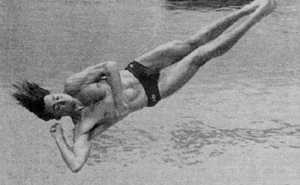
\includegraphics[width=6.5cm]{images/final-photo-2.png}\end{center}
照片摘自 MIT 8.012 Fall 2008 期末原件 PDF 第 5 页, 无单独第三方署名或许可例外标记; 沿用该 OCW 对象许可, 不声称本册原创照片.
\end{exercise}
\begin{solution}
(a) 内轨速率大, 比外轨 $\sqrt2$ 倍; 外轨角动量大, 为内轨 $2\sqrt2$ 倍. (b) 第三项. (c) 线动量与角动量守恒; 外力不做功并不保证人体的机械能守恒, 收臂有内部化学能转为转动动能. 如果“能量”指含内能的总能量, 则也守恒, 官方此题按机械能处理. (d) $[G]=L^3M^{-1}T^{-2}$. (e) 官方画引力与进动向量平行、同向斜右上. 以 $\vct r$ 向右、$\vct L$ 向左, 比较 $\vct r\times M\vct g=\vct\Omega\times\vct L$, 可确定 $\vct g$ 垂直轴的分量向上. 沿轴分量不产生力矩, 单由该方程不能定大小; 官方示意选择与进动平行的方向. (f) 官方依据伸展臂及头发方向判断前空翻, 同时有绕身体长轴的扭转, 角速度不是只沿画面法线的单一向量. 前空翻分量在图示中朝左上, 扭转分量大致沿躯干指向脚 (右上), 总向量从胸部朝较陡的右上, 为二者矢量和. 单张照片不能给这两个分量的数值比, 不把定性线索说成精确测量.
\begin{center}\begin{tikzpicture}[>=Latex]
\fill(0,0)circle(1.2pt);\node[below]at(0,0){胸部};
\draw[->,thick](0,0)--(-.8,1.4)node[left]{$\vct\omega_{flip}$};
\draw[->,thick](0,0)--(1.9,.8)node[right]{$\vct\omega_{twist}$};
\draw[->,very thick,color=structurecolor](0,0)--(1.1,2.2)node[above]{$\vct\omega_{total}$};
\node[below,align=center]at(.7,-.6){官方判断的方向示意\newline 长度为示意, 不是实测角速率};
\end{tikzpicture}\end{center}

\end{solution}
\begin{exercise}
原题 2. 固定滑轮是质量 $M$、半径 $R$ 的均匀盘, 轻绳无滑. 一端质量 $M$ 块悬在离地 $d$ 处, 一端质量 $2M$ 块在角 $\alpha$ 斜面, 摩擦系数 $\mu$. (a) 分别给悬块能上升或下降的条件. (b) 若悬块下降, 求加速度.
\end{exercise}
\begin{solution}
(a) 悬块下降需 $Mg>2Mg(\sin\alpha+\mu\cos\alpha)$; 上升需 $2Mg(\sin\alpha-\mu\cos\alpha)>Mg$. 其余区域在静摩擦模型中可保持静止. (b) 下为悬块正向, 写 $Mg-T_1=Ma,T_2-2Mg\sin\alpha-2\mu Mg\cos\alpha=2Ma,(T_1-T_2)R=(MR^2/2)a/R$. 相加得
\[a=\frac{2g}7(1-2\sin\alpha-2\mu\cos\alpha).\]
只适用轻块触地前的绷紧阶段; 高度 $d$ 不影响该恒加速度.
\end{solution}
\begin{exercise}
原题 3. 圆柱火箭直径 $2R$, 干质量 $M_R$, 初燃料 $M_F$, 以 $v_0$ 进入均匀静止粒子云. 数密度 $N$, 每粒质量 $m\ll M_R$. 后向排燃料速率 $\gamma>0$, 相对喷速 $u$, 忽略引力. (a) 阻力 $-Av^2$ 时写点火运动方程. (b) 保持 $v_0$ 的推力. (c) 突然耗尽燃料后的速率随时间. (d) Bonus: 鼻锥顶角 $90^\circ$, 每粒子弹性反射, 频繁连续撞击; 证明平方阻力并求 $A$.
\end{exercise}
\begin{solution}
(a) $M(t)=M_R+M_F-\gamma t$, $M(t)\dot v=\gamma u-Av^2$. 左侧不是 $\dd(Mv)/\dd t$, 后者需要显式包含流出动量. (b) $\gamma u=Av_0^2$. (c) 以耗尽时刻为 $t=0$, 当时速率 $v_b$, $M_R\dot v=-Av^2$, 故 $v=v_b/[1+(Av_b/M_R)t]$; 若此前一直维持速度则 $v_b=v_0$. (d) 火箭系入射相对速率 $v$, 在 $45^\circ$ 锥面弹性反射后纵向相对速度为零, 所以每粒纵向获得 $mv$. 每秒撞击 $N\pi R^2v$ 粒, 合力 $-Nm\pi R^2v^2$, 故 $A=Nm\pi R^2$. 对称锥面横向动量抵消. 若平鼻正面反射, 系数会多一个 2, 不是本题几何.
\end{solution}
\begin{exercise}
原题 4. 无摩擦桌上两均匀盘半径均 $R$, 上盘质量 $M$, 向右平移 $v_0$ 并逆时针自转 $\omega_0$; 下盘质量 $2M$, 静止. 上盘水平擦碰下盘顶端, 两中心连线在接触时竖直, 盘立即粘合. (a) 合体质心速度与转速的大小方向. (b) 哪个 $\omega_0$ 使合体不转? (c) 机械能损失.
\end{exercise}
\begin{solution}
(a) $V_C=v_0/3$ 向右. 上盘、下盘中心分别在合体质心上 $4R/3$、下 $2R/3$. 初角动量 $L_C=MR^2\omega_0/2-4MRv_0/3$, 合体惯量 $I_C=25MR^2/6$, 故
\[\omega_f=\frac{3R\omega_0-8v_0}{25R},\]
正为逆时针、负为顺时针. (b) $\omega_0=8v_0/(3R)$ 逆时针. (c) 原题未限制 (b) 情形, 一般损失
\[\Delta K_{\rm loss}=\frac13Mv_0^2+\frac14MR^2\omega_0^2-\frac{3L_C^2}{25MR^2}.\]
官方本小问额外按“合体不转”计算; 在 (b) 特例上述式为 $19Mv_0^2/9$. 本册给一般式后再列官方特例, 不把额外条件写回原题.
\end{solution}
\begin{exercise}
原题 5. 圆柱质量 $M$, 长 $L$, 半径 $R$, 轴水平沿 $+x$, 以 $\omega_s\uv x$ 自旋, 在无摩擦桌上. 在质心右侧轴向距离 $r$ 处给水平 $+y$ 冲量 $\Delta p$, $z$ 向上. (a) 碰后平移速度. (b) 角冲量远小于自旋角动量时, 倾角和哪端抬起. (c) 倾起后当作陀螺, 忽略章动, $R\ll L$, 求进动速率方向, 不必用欧拉方程. (d) Bonus: 强冲量可使进动反向, 最小倾角和所需最小冲量? 此问不能假定 $R\ll L$.
\end{exercise}
\begin{solution}
(a) $\vct V=\Delta p\uv y/M$. (b) $L_s=MR^2\omega_s/2$, $\Delta\vct L=r\Delta p\uv z$, 在小冲量快自旋近似中 $\alpha\simeq2r\Delta p/(MR^2\omega_s)$, 右端抬起. (c) 支承端到质心的水平力臂约 $L/2$, $\Omega L_s=MgL/2$, 故 $\vct\Omega\simeq Lg\uv z/(R^2\omega_s)$. 质心还可平移, 不妨碍关于质心的角动量平衡. (d) 完整几何力臂 $\ell=(L/2)\cos\alpha-R\sin\alpha$; 过零后重力矩反向, 临界 $\tan\alpha_c=L/(2R)$. 官方继续用 $\tan\alpha\simeq r\Delta p/L_s$ 估计 $\Delta p_c\simeq MRL\omega_s/(4r)$. 这把 (b) 小角冲量近似延伸到强冲量, 不是一般精确阈值. 倾角几何条件准确; 精确最小冲量需额外求碰撞后章动、接触、能量与有限进动角动量, 原题和官方短解未给这些完整条件. 不将近似估计冒充已证明的有限冲量定理.
\end{solution}
\begin{exercise}
原题 6. 无摩擦刚杆以恒角速度 $\omega$ 绕一端在平面旋转. 质量 $M$ 珠起初保持在距端 $r_0$, 径向静止, 忽略重力. (a) 保持它所需力大小方向. (b) 释放后的惯性极坐标位置. (c) 杆系惯性力及杆在两系中所给真实力.
\end{exercise}
\begin{solution}
(a) 径向保持力 $-M\omega^2r_0\uv r$, 此时无横向杆力. (b) $\theta=\theta_0+\omega t$, 径向方程 $\ddot r-\omega^2r=0$, 初条件给 $r=r_0\cosh\omega t$. (c) 杆系离心力 $M\omega^2r\uv r$, 科里奥利力 $-2M\omega\dot r\uv\theta$; 真实杆约束力与后者抵消, 为 $2M\omega\dot r\uv\theta=2M\omega^2r_0\sinh\omega t\uv\theta$. 惯性系中同一真实力提供 $a_\theta=2\omega\dot r$. 两系答案必须是同一物理力.
\end{solution}
\begin{exercise}
原题 7. 质量 $m$ 质点受中心力 $\vct F=-Ar^3\uv r$, $A>0$, 初在 $r_0$ 以纯切向速率 $v_0$ 运动. (a) 推导并画有效势, 标明重要转折点; 原文称“inflection points”. 能否经过原点? (b) 在 $r_0$ 作圆轨道所需速率. (c) 圆轨道附近小径向振荡频率及其周期与公转周期比较.
\end{exercise}
\begin{solution}
(a) $L=mr_0v_0$, $U=Ar^4/4$, $U_{eff}=Ar^4/4+L^2/(2mr^2)$. $L\ne0$ 时两端均趋 $+\infty$, 唯一极小点 $r_e=(L^2/(mA))^{1/6}$. $U_{eff}''=3Ar^2+3L^2/(mr^4)>0$, 因此没有数学意义的拐点; 此处更正原词为势阱极小点. $L\ne0$ 的离心势垒阻止到原点, $v_0=0$ 则无此势垒, 可径向穿过. 下图取单位化 $A=m=L=1$.
\begin{center}\begin{tikzpicture}\begin{axis}[width=7.4cm,height=4.4cm,xmin=.3,xmax=2,ymin=0,ymax=5,axis lines=left,xlabel={$r/r_e$},ylabel={$U_{eff}/(Ar_e^4)$},samples=120]
\addplot[thick,domain=.33:1.9]{x^4/4+1/(2*x^2)};
\addplot[dashed,domain=.3:1.9]{.75};\node[above]at(axis cs:1,.75){极小点};
\end{axis}\end{tikzpicture}\end{center}
(b) $mv_c^2/r_0=Ar_0^3$, 所以 $v_c=r_0^2\sqrt{A/m}$. (c) 令 $r=r_0+\xi$, $m\ddot\xi=-U_{eff}''(r_0)\xi=-6Ar_0^2\xi$, 故角频率 $\omega_r=\sqrt{6Ar_0^2/m}$, 普通频率 $f_r=\omega_r/(2\pi)$. 公转角频率 $\omega_{orb}=v_c/r_0=\sqrt{Ar_0^2/m}$, 周期比 $T_r/T_{orb}=1/\sqrt6$. 数值轨迹复现见项目, 不以数值代替线性化证明.
\end{solution}

\originalsection{官方公式表的中文对照}
三份独立期中公式表及期末末页所列公式在此合并, 重复条目只出现一次. 符号与正文一致: $\vct R$ 是质心位置, $I_C$ 是质心惯量, $\vct\Omega$ 是参考系角速度, $\vct a_0$ 是系原点加速度. 该对照保留适用条件, 不改变原考试允许查表的范围.
\begin{align*}
\vct v&=\dot r\uv r+r\dot\theta\uv\theta,&
\vct a&=(\ddot r-r\dot\theta^2)\uv r+(r\ddot\theta+2\dot r\dot\theta)\uv\theta,\\
\vct R&=M^{-1}\int\vct r\dd m,&\dd V&=r\dd r\dd\theta\dd z,\\
K&=\tfrac12mv^2,&W&=\int\vct F\cdot\dd\vct r,\\
U_B-U_A&=-\int_A^B\vct F\cdot\dd\vct r,&\vct L&=\vct r\times\vct p,\\
\vct\tau&=\vct r\times\vct F,&\tau_z&=I_z\alpha_z\quad\text{(固定主轴)},\\
I_O&=I_C+Md^2,&I_{ij}&=\int(r^2\delta_{ij}-x_ix_j)\dd m.
\end{align*}
常加速度轨迹 $\vct r(t)=\vct r_0+\vct v_0t+\vct a t^2/2$, 牛顿引力 $\vct F=-GMm\uv r/r^2$, 笛卡尔体积元 $\dd V=\dd x\dd y\dd z$, 质点动能定理 $K_B-K_A=W_{net}$. 这些与前述极坐标、功和势能式分别对应, 不能漏掉常加速度的初条件项.

均匀杆中点垂直轴 $ML^2/12$, 薄环对称轴 $MR^2$, 盘对称轴 $MR^2/2$, 实心球直径轴 $2MR^2/5$. 原表张量公式以 $xx$ 为例并允许循环置换, 完整 $I_{ij}$ 为本册展开; 欧拉方程为 $I_1\dot\omega_1+(I_3-I_2)\omega_2\omega_3=\tau_1$ 及两循环式. 导数变换 $({\dd\vct A}/{\dd t})_I=({\dd\vct A}/{\dd t})_R+\vct\Omega\times\vct A$; 加速系惯性力 $-m\vct a_0$, 恒角速旋转系再有 $-2m\vct\Omega\times\vct v_R-m\vct\Omega\times(\vct\Omega\times\vct r)$. 泰勒展开 $f(x+h)=f(x)+hf'(x)+h^2f''(x)/2+\cdots$. 非恒 $\Omega$ 的欧拉惯性力属于正文补充, 不是把它伪装成原表项目.

刚体动能 $K=MV_C^2/2+\vct\omega\cdot I_C\vct\omega/2$, 角动量关系 $\vct L_C=I_C\vct\omega$, 固定惯性参考点的力矩式 $\vct\tau=\dd\vct L/\dd t$, 固定轴的转动功 $W=\int\tau_z\dd\theta$. 保守力 $\vct F_c=-\nabla U$, 在单连通光滑区域可用 $\nabla\times\vct F_c=0$ 判定. 期中二公式表原把 $W=\Delta E=\Delta(K+U)=\int\vct F\cdot\dd\vct r$ 并列; 当 $\vct F$ 是净力时正确的是 $W_{net}=\Delta K$, 而包括保守势能后应把对应保守力功移至势能端. 本册在此明确更正, 不沿袭原表混淆.
